\begin{frame}
    \begin{centering}
        \vskip5ex plus 1filll
        {\usebeamerfont{title page title}\usebeamercolor[fg]{title page} Real-Time Implementation\\[1.5ex]}
        \vskip0pt plus 1filll
    \end{centering}
\end{frame}

\begin{frame}{Klon Centaur Circuit Schematic}
    \begin{figure}
        \centering
        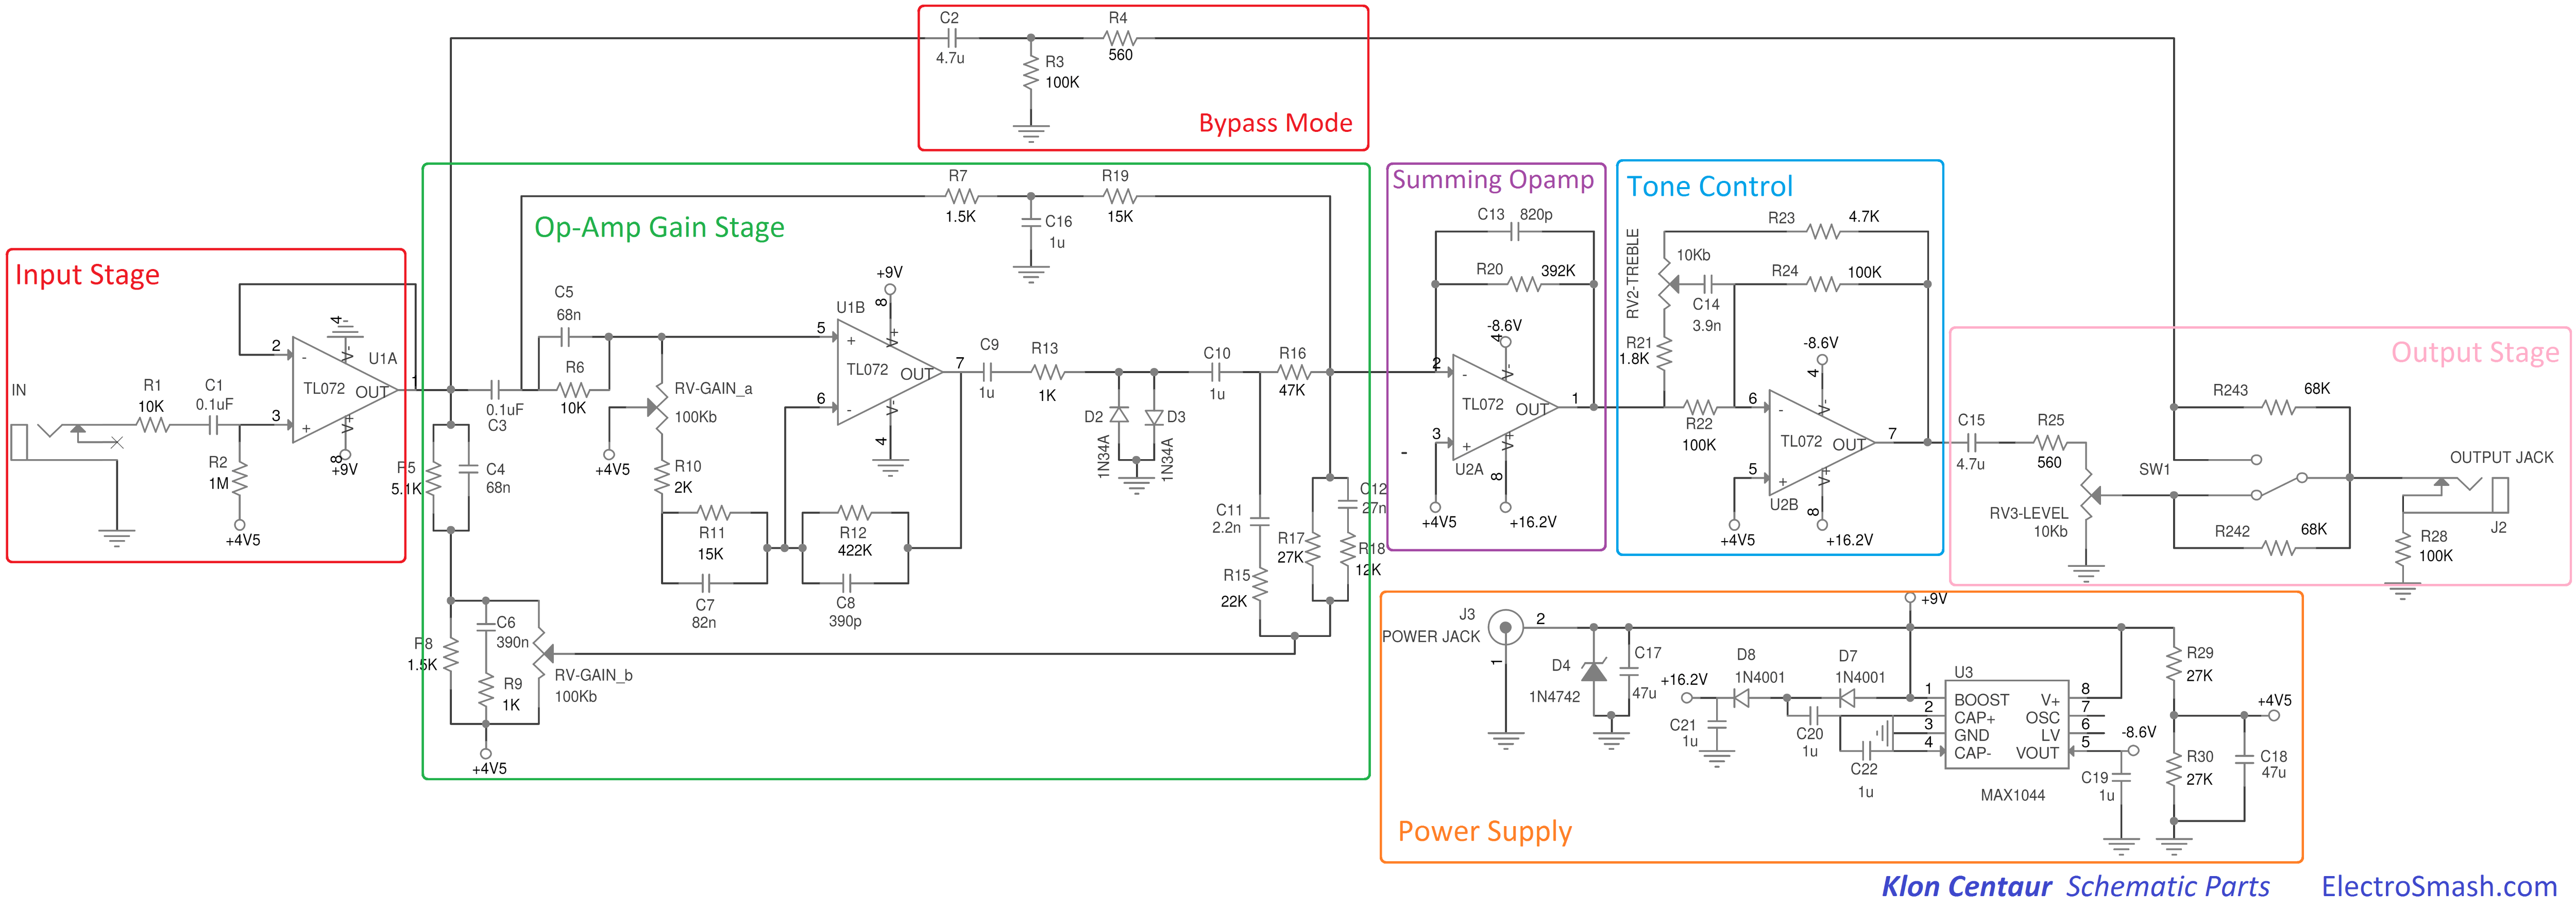
\includegraphics[width=5.75in]{../Paper/Figures/FullCircuit.png}
    \end{figure}
\end{frame}

\begin{frame}{Implementation}
    \begin{columns}
        \begin{column}{0.45\linewidth}
            Non-ML Implementation
            \begin{itemize}
                \item Use a combination nodal analysis, WDFs
                \item Control parameters for Treble, Gain, Level
            \end{itemize}
        \end{column}
        \begin{column}{0.55\linewidth}
            ML Implementation
            \begin{itemize}
                \item RNN model for Gain Stage, nodal analysis elsewhere
                \item Fade between models for variable Gain control
                \item Custom GRU and Dense layer implementations in C++
            \end{itemize}
        \end{column}
    \end{columns}
\end{frame}

\begin{frame}{RNN Inferencing Engine}
    Tensorflow Lite
    \begin{itemize}
        \item Converts a Tensorflow model to a format that can be run on embedded devices
        \item Support for GRUs is still experimental
        \item Real-time audio concerns: no thread locks, no memory allocation on real-time audio thread
    \end{itemize}
\end{frame}

\begin{frame}{RNN Inferencing Engine}
    Custom engine: Eigen
    \begin{itemize}
        \item Eigen is a linear algebra C++ library with SIMD support for matrix/vector operations
        \item Custom implementations of GRU and fully connected layers, validated against Tensorflow
        \item Can be difficult to compile on embedded devices
    \end{itemize}
\end{frame}

\begin{frame}{RNN Inferencing Engine}
    Custom engine: C++ STL
    \begin{itemize}
        \item Optimized algorithms for operations such as \lstinline{std::inner_product}
        \item Custom implementations of GRU and fully connected layers, validated against Tensorflow
        \item Can be compiled on most embedded devices
    \end{itemize}
\end{frame}

\begin{frame}{Implementation}
    Desktop Audio Plugin (JUCE/C++)
    \begin{figure}
        \centering
        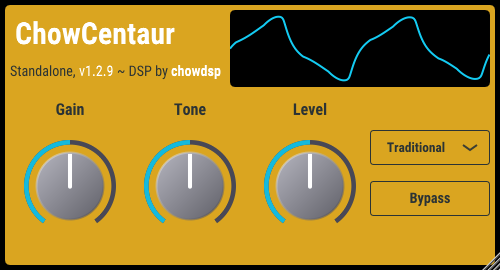
\includegraphics[height=2.5in]{../Paper/Figures/Plugin.png}
    \end{figure}
\end{frame}

\begin{frame}{Implementation}
    Teensy 4.0, Teensy Audio Shield, Teensy Audio Library
    \begin{figure}
        \centering
        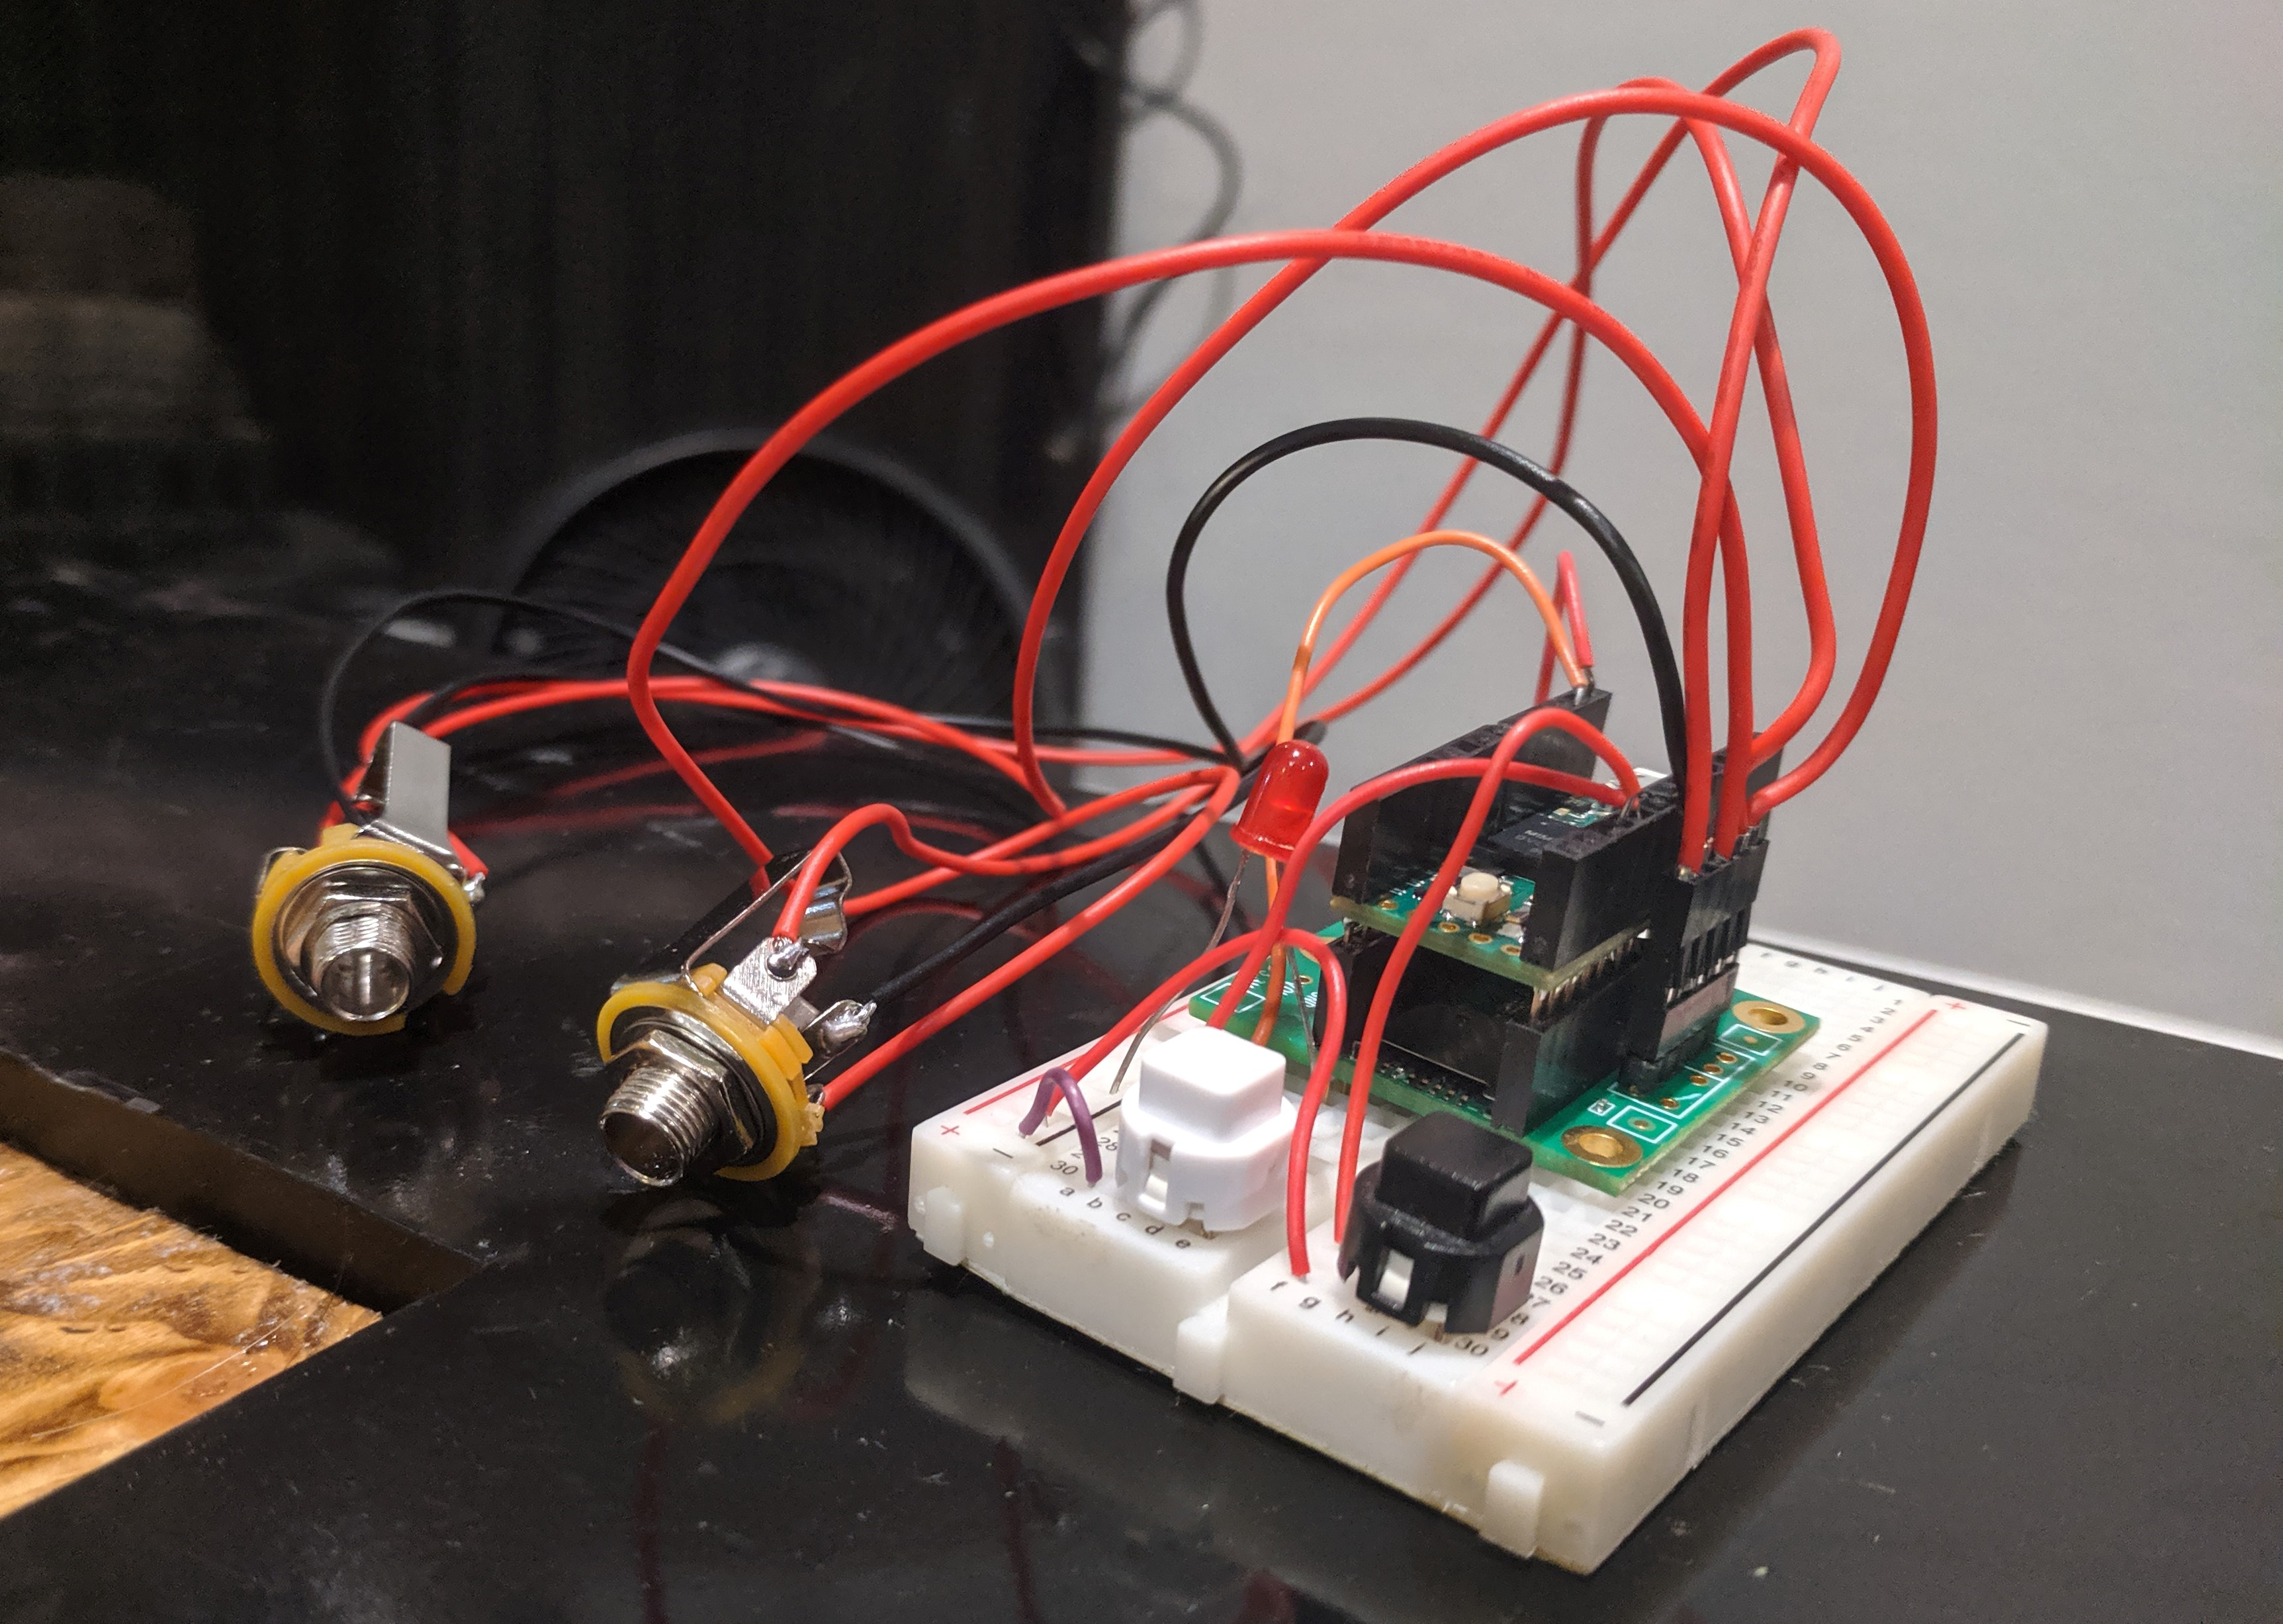
\includegraphics[height=2.5in]{../Paper/Figures/Teensy.jpg}
    \end{figure}
\end{frame}

\begin{frame}{Results: Performance}
    Compute time per second of audio.
    \begin{table}[h!]
        \centering
         \begin{tabular}{||c | c | c||} 
         \hline
         Block Size & NonML Speed & ML Speed \\
         \hline\hline
         8    & 0.0723437 & 0.0528792 \\
         16   & 0.0703079 & 0.0510437 \\
         32   & 0.0652856 & 0.0511147 \\
         64   & 0.0662835 & 0.0502434 \\
         128  & 0.0666593 & 0.0495194 \\
         256  & 0.0696844 & 0.0480298 \\
         512  & 0.0669037 & 0.0477946 \\
         1024 & 0.060816  & 0.0488841 \\
         2048 & 0.0695175 & 0.0488309 \\
         4096 & 0.0623839 & 0.0472191 \\
         \hline
         \end{tabular}
    \end{table}
\end{frame}

\begin{frame}{Results: Summary}
    \begin{itemize}
        \item Subjectively, non-ML and ML models sound very similar.
        \item ML model has slightly damped high frequency response,
            (not a big deal on guitar input; more noticeable on other audio).
        \item ML model is more efficient!
    \end{itemize}
\end{frame}

\begin{frame}{Takeaways}
    \begin{itemize}
        \itemsep0.75em
        \item 3 methods for modelling circuits:
        \begin{itemize}
            \item Nodal Analysis (simplest)
            \item Wave Digital Filters (modular)
            \item Neural Networks (experimental)
        \end{itemize}
        \item Modelling circuits with neural networks can be done, but more research/experimentation is needed
        \item Desktop vs. Embedded:
        \begin{itemize}
            \item Memory management
            \item Processing power (floating point processing, SIMD)
            \item Price
        \end{itemize}
    \end{itemize}
\end{frame}
